\section{Experimental Setup}
We use  \texttt{Llama-3.1-8B-Instruct}, \texttt{google/gemma\\-7b-it}, and \texttt{mistralai/Mistral-7B-Instruct-\\v0.3} as they are open-source instruction tuned models~\cite{grattafiori2024llama3herdmodels,gemmateam2024gemmaopenmodelsbased}. We opt to use smaller models for broader accessibility and lower computational costs. We compare the ability of the control vector methods to In-Context Learning (ICL), Supervised Fine Tuning (SFT), LoRa/QLoRa SFT and DSPy Prompt Optimization. ICL has shown great abilities in instruction following, and is a similarly low data, lightweight method~\cite{Brown2020LanguageMA}. For ICL, we take a positive and negative example from the extraction set (\S\ref{sec:data-selection}) as examples of a lay summary and technical summary, respectively. We then provide the document to the model and ask it to summarize the document with a specified readability level. We repeat this with 5 levels of specified readability.SFT and QLoRa/LoRa SFT based methods \cite{hu2021loralowrankadaptationlarge, dettmers2023qloraefficientfinetuningquantized}.  Prompt Optimization has shown promise as a way to control language models without expensive training \cite{khattab2023dspycompilingdeclarativelanguage}.   See \S\ref{appendix:cv-details} and \S\ref{appendix:base-details} for additional details.

Past work has shown that the Coleman-Liau readability index (CLI)~\cite{Coleman1975ACR} and Dale-Chall readability scores (DCRS)~\cite{dale1948formula} correlate the highest with human judgments of readability~\cite{Cachola2025EvaluatingTE}. To avoid overfitting to our evaluation, we use DCRS for our data selection (\S\ref{sec:data-selection}) and CLI for our system evaluation (\S\ref{sec:4-chapter-results}). To evaluate system performance, we report the Pearson~\cite{PearsonVIINO} and Kendall-Tau~\cite{Kendall1938ANM} correlation of the specific strength scalar with CLI. CLI provides a lower score for higher readability, while our setup treats the lay summary as the positive example. In other words, we expect higher control vector strengths to produce lower CLI scores. Therefore, we multiply the CLI scores by $-1$ so the resulting correlations are positive. We also use BERTScore \cite{Zhang2019BERTScoreET} with the abstract as the reference, since some dataset lay summaries contain extraneous information not present in the original document and thus make poor evaluation references.

\section{Meeting Data Requirements}\label{sec:data-selection}

We begin with four different scientific summarization datasets: eLife~\cite{Goldsack2022MakingSS}, Eureka~\cite{Zaman2020HTSSAN}, PLOS~\cite{Goldsack2022MakingSS}, and SciNews~\cite{pu-etal-2024-scinews}. These datasets are designed for  scientific PLS, allowing us to use the lay summary as the positive example and the abstract as the technical, negative example. Additional dataset descriptions in~\S\ref{appendix:dataset-details}.

% meet 2 requirements: (1) The positive and negative examples must be sufficiently different in readability and (2) The positive and negative examples must have approximately the same content, only differing in their readability level.


We choose an extraction dataset that follows the requirements outlined in~\S\ref{sec:4-chapter-method}. Req. 1 states that the paired examples must be sufficiently different in readability. We plot the Dale-Chall scores of the positive and negative examples for each dataset in a histogram. We additionally calculate the Bhattacharyya distance, which measures the overlap between two distributions~\cite{Bhattacharyya1943OnAM}. A dataset that best meets this requirement will have a large visual separation between the two distributions, as well as a high Bhattacharyya distance. \Cref{fig:dale-chall-hists} contains both the histograms and the Bhattacharyya distance for each dataset. eLife has both the highest visual separation and highest Bhattacharyya distance. PLOS has a particularly low separation, indicating that the PLOS lay summaries are not significantly more readable than the technical summaries.
\begin{figure}[!ht]
    \vspace{-3mm}
    \centering
    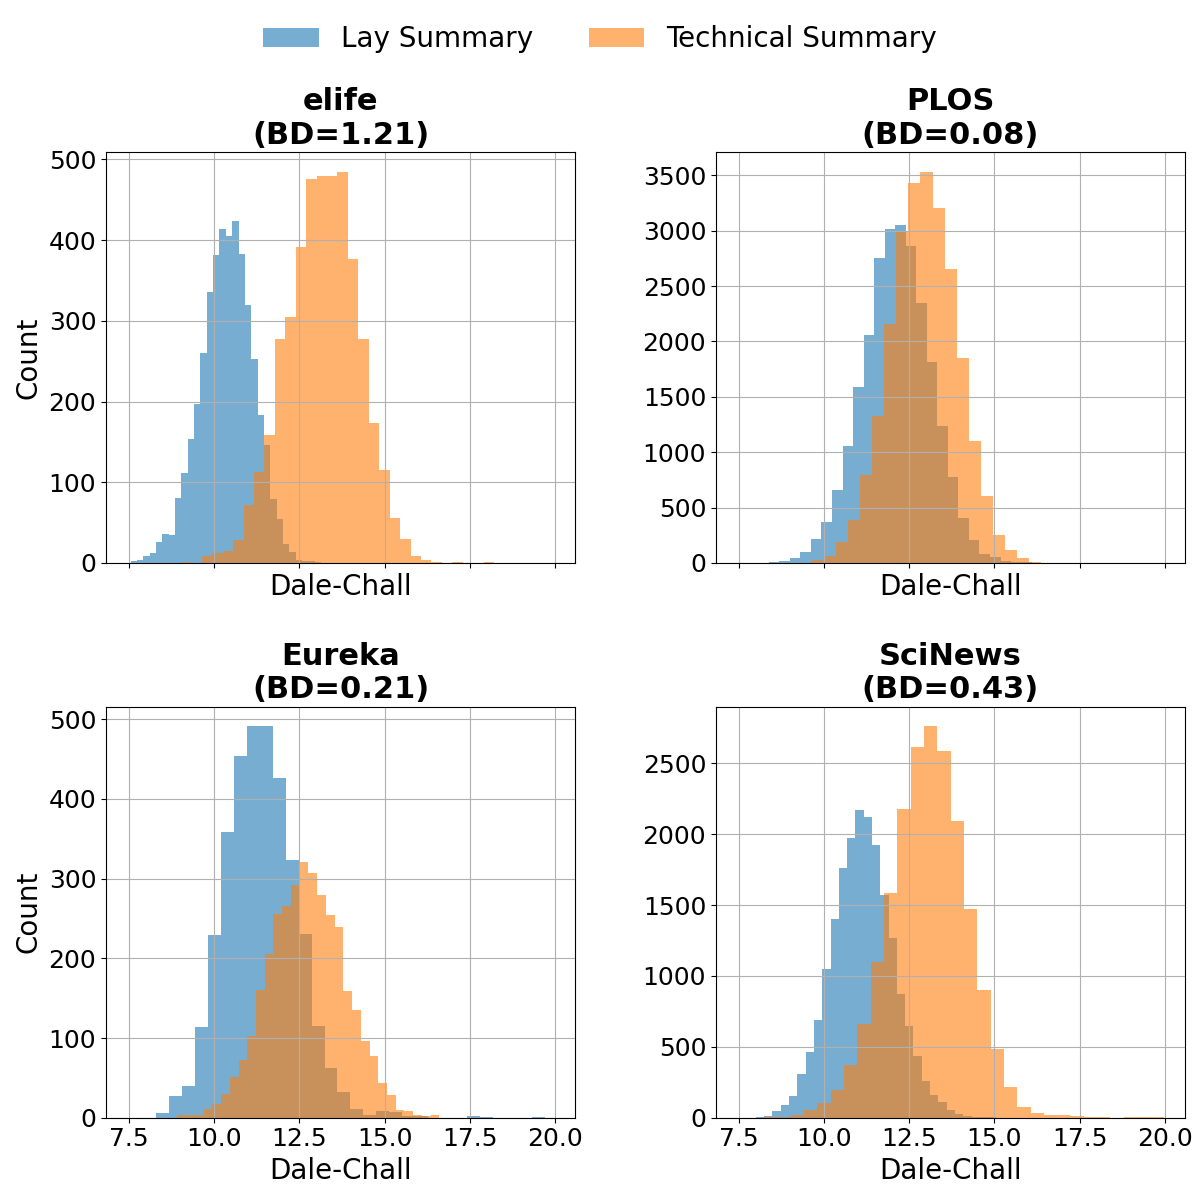
\includegraphics[width=.9\linewidth]{research-chapters/4-chapter/figures/dale_chall_histograms.png}
    \vspace{-3mm}
    \caption{Histogram of the Dale-Chall readability scores for the lay and technical summaries and the Bhattacharyya distance (BD) of each dataset.}
    \label{fig:dale-chall-hists}
    \vspace{-5mm}
\end{figure}

Req. 2 states that the positive and negative examples must have approximately the same content, only differing in their readability level. In order to measure overlap in content, we use Sentence Transformers to retrieve an embedding matrix for the example pairs, then compute the cosine similarity~\cite{reimers-gurevych-2019-sentence}. We use Specter for the embeddings, a model trained on scientific data~\cite{cohan-etal-2020-specter}. The resulting mean cosine similarity scores are as follows: $0.631$ for eLife, $0.604$ for PLOS, $0.575$ for Eureka, and $0.590$ for SciNews. Based on these scores, we conclude that eLife and PLOS have the highest content similarity while Eureka and SciNews have the lowest. This aligns from the construction of the datasets: eLife and PLOS's lay summaries written by the original paper authors to be accessible explanations of their papers while Eureka and SciNews's summaries are news reports discussing papers. Upon inspection, we find that Eureka and SciNews often contain information not present in the abstract, such as interviews with the authors or information on a study's funding source. We provide examples from each dataset in~\S\ref{appendix:dataset-examples}.
Based on this analysis, we conclude that eLife best meets the requirements. As the control vector method does not require a large extraction dataset, we select 128 of the most readable examples (lowest Dale-Chall) from the eLife training set. Choosing the most readable examples gives the control vectors the best examples of readability. We use this setup to report our main results in~\S\ref{sec:4-chapter-results}. 


